\documentclass[aspectratio=169]{beamer}

\usepackage[utf8]{inputenc}
\usepackage{default}
\usepackage[spanish]{babel}
\usepackage{amsmath}
\usepackage{amsfonts}
\usepackage{amssymb}
\usepackage{subfig}
\usepackage{tabto}
% 

\begin{document}


\title{\textbf{Sistema de transmisión segura punto a punto y multipunto en medios compartidos.}}


\author{\small Alfredo Adrián Ortega\\
Instituto Tecnológico de Buenos Aires (ITBA) \\
     aortega@itba.edu.ar\\    }





\frame{\titlepage

\begin{columns}
  \begin{column}{0.99\textwidth}

\begin{figure}[h]
  \centering
    \hspace{0.8cm} 
\includegraphics[height=0.7cm]{graphs/ITBA_sfondo2.png}
\end{figure}

  \end{column}

  \begin{column}{0.01\textwidth}

  \end{column}
\end{columns}
}

%% TOC

\frame{\frametitle{Contenido}\tableofcontents[hideallsubsections]}

\section{Motivación}

\begin{frame}{Motivación}

\begin{itemize}
 \item Lograr privacidad a nivel físico en comunicaciones digitales.
 \item El costo de las intrusiones y robo de datos en el 2011 en EEUU ascendió en promedio a 5.5 us\$ millones por organización (Symantec).
 \item Facilidad de robo de datos en medios compartidos.
 \item Productos comerciales (ID Quantique, NuCrypt, etc.) intentan solucionar este tipo de problemas. 
 \end{itemize}

% \begin{figure}[t]
%  \centering
%  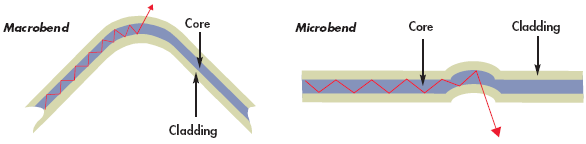
\includegraphics[width=0.75 \textwidth]{graphs/microbend.png}
  
%  Fugas por Microbend y macrobend en fibra óptica \cite{jay2010}
%\end{figure}

\end{frame}


\begin{frame}{Robo de datos en fibras ópticas}

\begin{itemize}
 \item Privacidad de datos en una red que utiliza un medio compartido.
 \item Protección ante nodos maliciosos. 
 \item Eliminar toda fuga de información.
 \end{itemize}

 \begin{figure}[t]
  \centering
  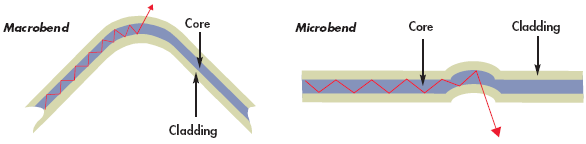
\includegraphics[width=0.75 \textwidth]{graphs/microbend.png}
  
  Fugas por Microbend y macrobend en fibra óptica \cite{jay2010}
\end{figure}

\end{frame}

%------------------------------------------------------------


%------------------------------------------------------------

\begin{frame}{Robo de datos en fibras ópticas}
\begin{figure}[t]
  \centering
  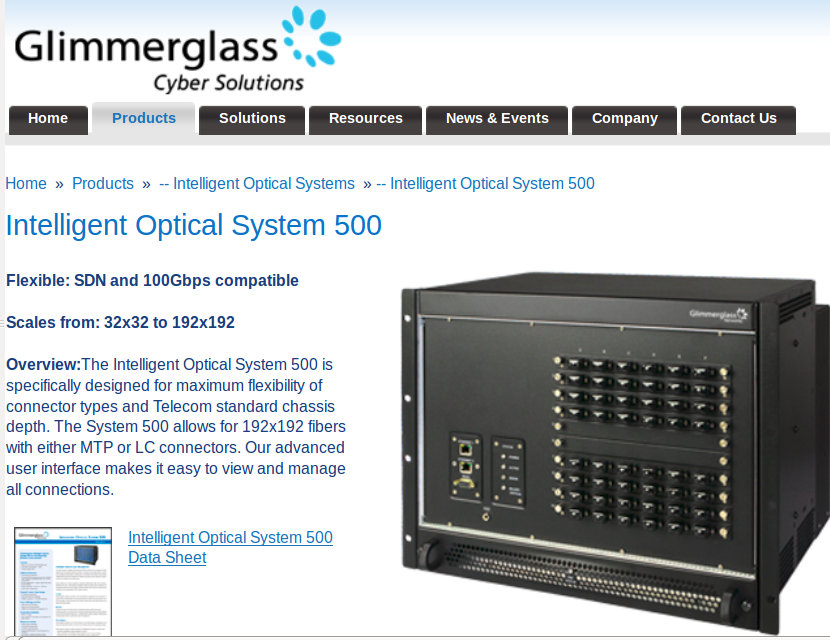
\includegraphics[width=0.75 \textwidth]{graphs/glimmer1.jpg} 
\end{figure}
\end{frame}

%------------------------------------------------------------


\begin{frame}{Robo de datos en fibras ópticas}
\begin{figure}[t]
  \centering
  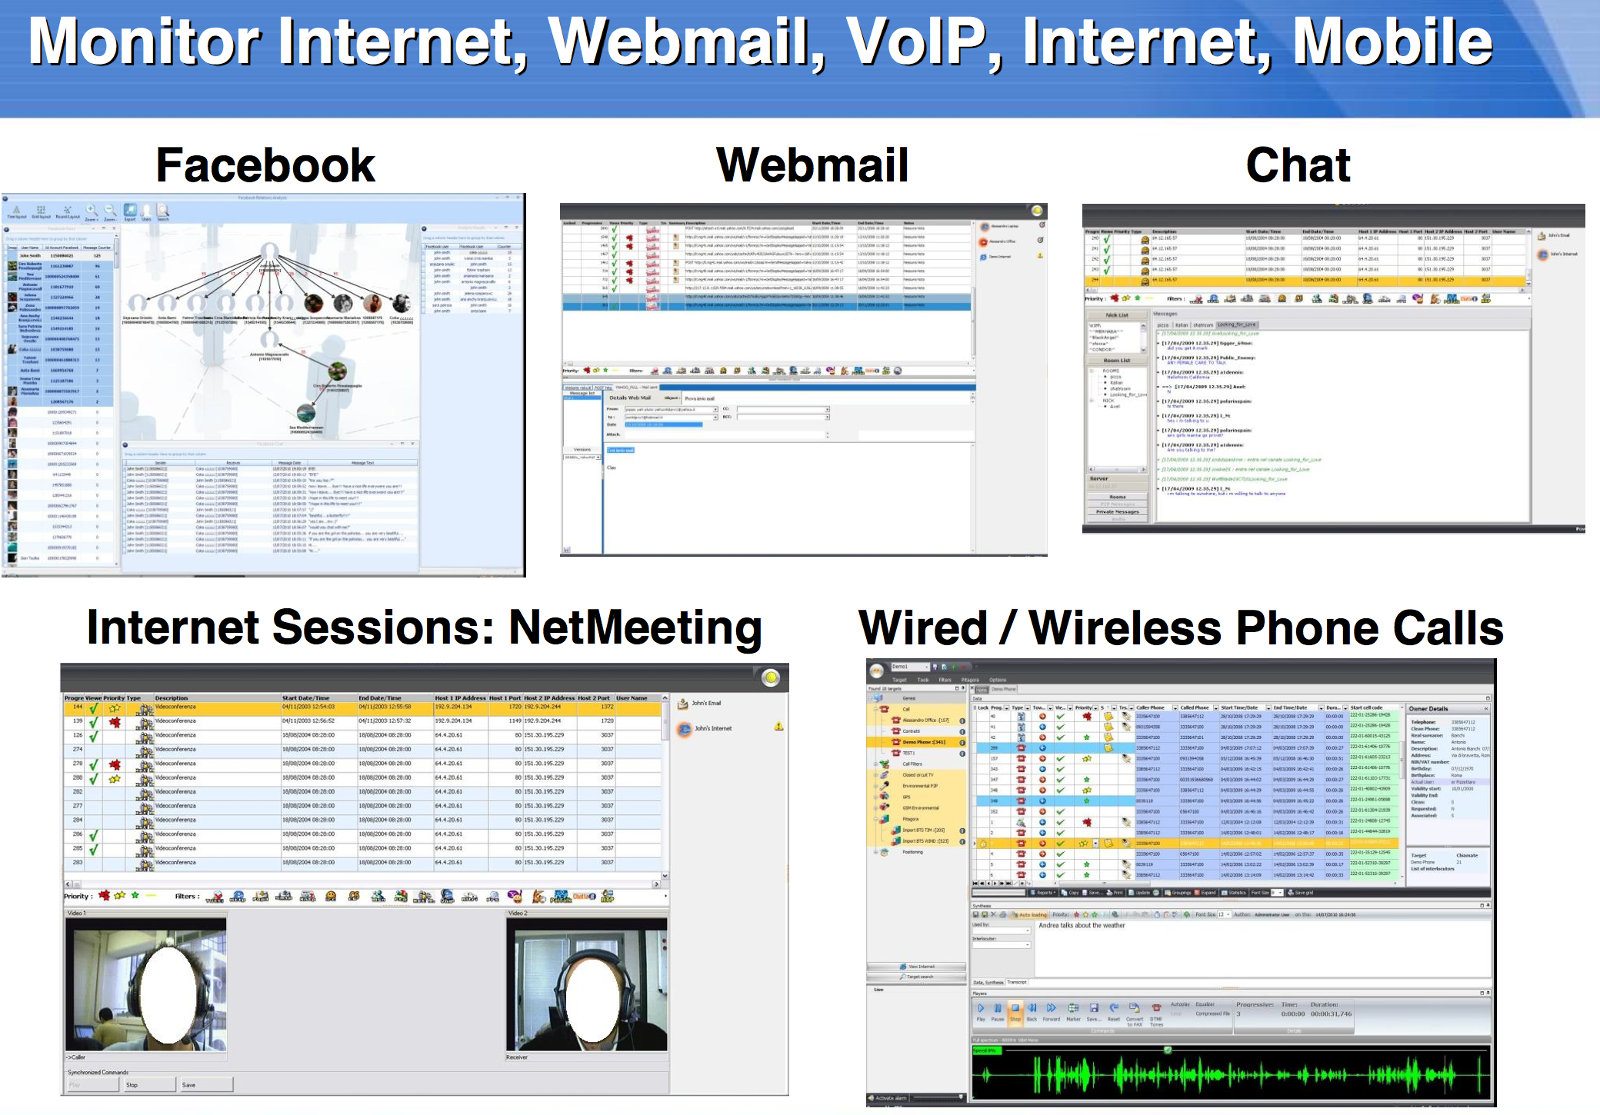
\includegraphics[width=0.80 \textwidth]{graphs/glimmer2.jpg} 
\end{figure}
\end{frame}

%------------------------------------------------------------

\begin{frame}{Privacidad en redes acústicas}

\begin{itemize}
 \item Transmisión segura de claves/contacto/sistemas de TFA.
 \item Transacciones comerciales a corta distancia.
 \item Reemplazo de NFC, sin hardware específico.
 \item Ej. Google tone: \textit{``An experimental chrome extension for instant sharing over au-
dio''}
 \end{itemize}
 
 \begin{figure}[t]
  \centering
  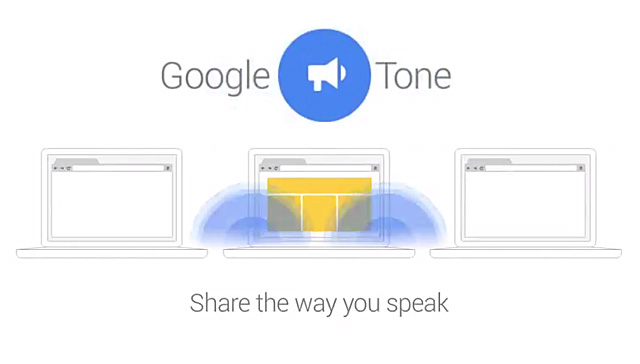
\includegraphics[width=0.65 \textwidth]{graphs/google_tone.jpg} 
\end{figure}
\end{frame}


%------------------------------------------------------------

\begin{frame}{Red pública con privacidad}

\begin{enumerate}
 \item Red: enlaces punto-a-punto y multipunto.
 \item Privacidad: nivel físico, criptográficamente fuerte.
 \item CDMA: acceso asincrónico sin control centralizado.
 \item Diferentes medios:
 \begin{enumerate}
 \item Guiados: Fibra óptica
 \item No guiados: Electromagnético y acústico.
\end{enumerate}
 
\end{enumerate}

\end{frame}
%------------------------------------------------------------

\begin{frame}{Desafíos en medios acústicos y fibra óptica}
\begin{columns}
  \begin{column}{0.60\textwidth}

\begin{enumerate}
 \item Evitar protocolos de control que debiliten la criptografía
 \item Aislación completa de canales de comunicación, para evitar ataques del tipo \textit{side channel}.
 \item Bajo costo - utilización de hardware pre-existente.
 \item Fibra óptica: Sistema capaz de operar a 5 Gbps+ 
 \item Medio acústico: Bajo consumo de potencia y alta frecuencia de portadora.
 \end{enumerate}

  \end{column}
  \begin{column}{0.40\textwidth}
 
 
 \begin{figure}[!t]
   \centering
   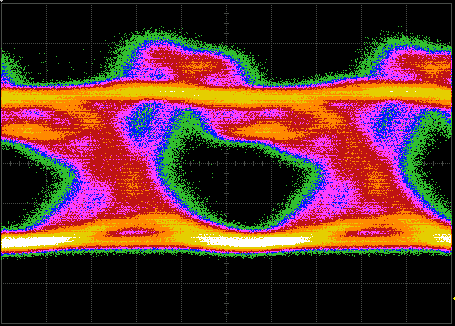
\includegraphics[width=0.80 \textwidth]{../graphs/medicionesPaper/eye71G.png}
   \qquad
   Diagramas de ojo, tasa de $7.5$ Gbps, 20 ns por división.
%  \caption {Diagramas de ojo, tasa de $7.5$ Gbps, 20 ns por división.}
  \label{fig:ImgOjo}
\end{figure}


\end{column}
\end{columns}

\end{frame}

%-------------------------------------------------------------

\section{Estado del Arte}
\frame{\tableofcontents[currentsection]}

\frame{\frametitle{Seguridad en las capas de red}
%\framesubtitle{ Capas de red}

\begin{columns}
  \begin{column}{0.40\textwidth}

\begin{figure}[t]
  \centering
    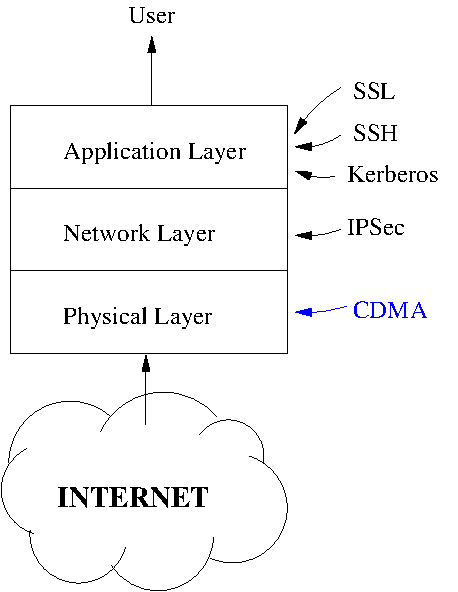
\includegraphics[width=0.80\textwidth]{graphs/layers.pdf}
    \\ Modelo de red OSI simplificado
    \label{ios_process_mem}
\end{figure}

  \end{column}
  \begin{column}{0.65\textwidth}

  \begin{itemize}
      \item SSH - solo punto-a-punto.
      \item SSL - protocolo muy complejo, muchas vulnerabilidades.
      \item IPSEC - poco difundido, configuración compleja
      \item Kerberos - idem SSL.
  \end{itemize}
  \pause\vfill
  {\bf Desventajas:}
	  \begin{itemize}
	  \item Complejidad y vulnerabilidades de \alert{implementación}.
	  \item Problemas en la \alert{configuración}.
	  \end{itemize}	  

  \end{column}
\end{columns}

}


\frame{
\frametitle{Seguridad en las capas de red}

\begin{columns}
  \begin{column}{0.40\textwidth}

\begin{figure}[t]
  \centering
    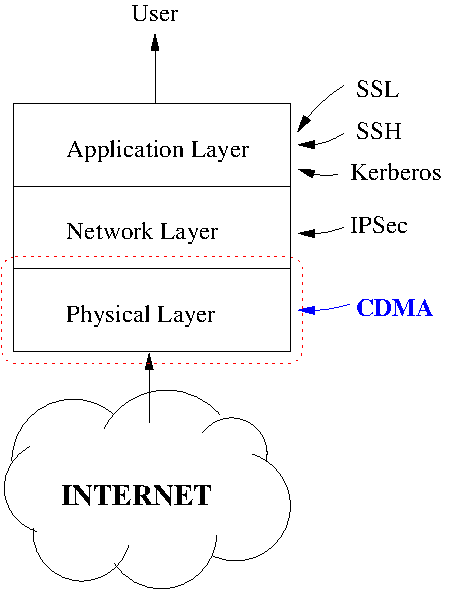
\includegraphics[width=0.80\textwidth]{graphs/layers2.pdf}
    \\ Modelo de red OSI simplificado
    \label{ios_process_mem}
\end{figure}

  \end{column}
  \begin{column}{0.65\textwidth}

  \begin{itemize}

    \item Reflectores de tipo red de Bragg (\textit{Bragg Grating}) \cite{torres2002}
	  \begin{itemize}
	  \item Configuración \alert{fija}
	  \end{itemize}

    \vfill\pause
	  
    \item Sistema propuesto en~\cite{mosso2011all}
	\begin{itemize}
	\item Baja cantidad de canales (\alert{crosstalk})
	\item Espacio de claves \alert{reducido}
     \end{itemize}
     
     \vfill\pause
	  
    \item CDMA \& códigos Walsh-Hadamard \cite{Nadarajah2006}
	  \begin{itemize}
	  \item Perfectamente ortogonales.
	  \item Espacio de claves \alert{muy reducido} \cite{Shake:05}
	  \end{itemize}
	
      \end{itemize}

  \end{column}
\end{columns}

}


%\frame{\frametitle{Security in the layered network model}


%\begin{itemize}

% \item Aplying Advanced Encryption Standard (AES, see~\cite{Daemen98aesproposal:}) to data, then sent by direct sequence CDMA with a short code% ength~\cite{Wang:10}.
% \begin{itemize}
% \item Altough this method offers privacy and high channel utilisation, it is limited to point-to-point communication. % vb 121122
% \end{itemize}
%\end{itemize}

%}

\section{Sistema propuesto}
\frame{\tableofcontents[currentsection]}

\frame{\frametitle{Sistema propuesto}
\vfill
\textbf{Basado en:}
\begin{itemize}
 \item{Medio de tipo bróadcast, modelado como canal Z}
 \item{Utilización de CDMA}
 \item{Corrección de errores optimizada para el tipo de canal}
 %\item[Time-hopping Spread Spectrum:] El tiempo de transmisión se selecciona mediante un algoritmo generador de números pseudoaleatorios (\alert{PRBS}).
 %\item[Filtro de Bloom:] Provee \alert{corrección de errores} asimétrica (en un canal Z)\vfill
 %\item[Minimización de peso de Hamming:] \alert{reducción} de símbolos problemáticos en el canal Z\vfill
\end{itemize}
\vfill
\pause
\textbf{Ventajas:}
  \begin{itemize}
  \item Punto-a-punto y Punto-a-\alert{multipunto}\vfill
  \item \alert{Privacidad}\vfill
  \end{itemize}
\vfill
}


%-------------------------------------------------------------

\subsection{Metodología}
\frame{\tableofcontents[currentsection,currentsubsection]}

%------------------------------------------------------------
\subsection{Canal Z}

\begin{frame}{Canal Z}
\begin{figure}[t]
  \centering
    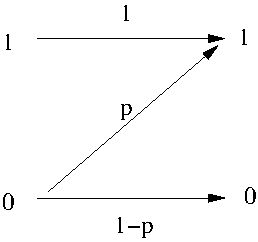
\includegraphics[width=5cm]{../graphs/zchannel.pdf}
    
    Diagrama de probabilidad del canal binario asimétrico o canal Z, donde p es la probabilidad de error.
\end{figure}
\end{frame}

%------------------------------------------------------------
\subsection{CDMA Time hopping}
\frame{\tableofcontents[currentsection,currentsubsection]}

\begin{frame}{Selección de casillero aleatoria: \textit{time hopping}}
\begin{figure}[t]
  \centering
    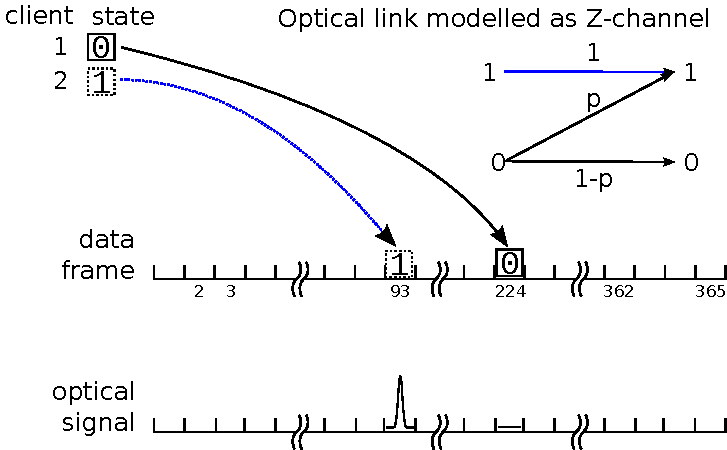
\includegraphics[width=8cm]{graphs/slide2.pdf}
    \\ \huge No hay colisión
\end{figure}
\end{frame}
%------------------------------------------------------------
\begin{frame}{Selección de casillero aleatoria: \textit{time hopping}}
\begin{figure}[t]
  \centering
    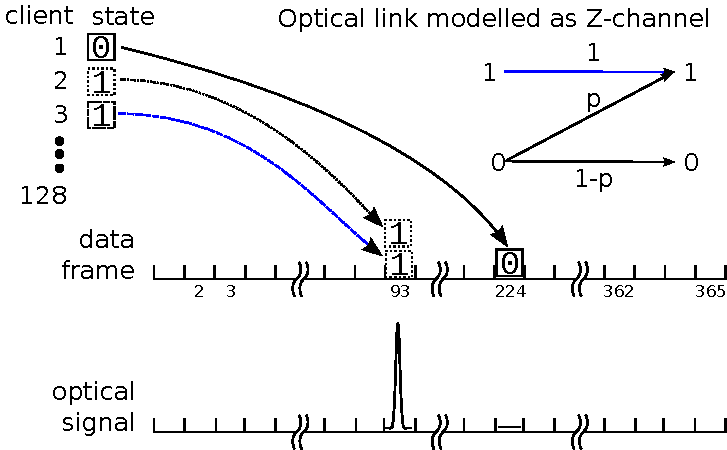
\includegraphics[width=8cm]{graphs/slide3.pdf}
    \\ \huge Colisión $\Rightarrow$ \textcolor{blue}{Resultado OK}
\end{figure}
\end{frame}
%------------------------------------------------------------
\begin{frame}{Selección de casillero aleatoria: \textit{time hopping}}
\begin{figure}[t]
  \centering
    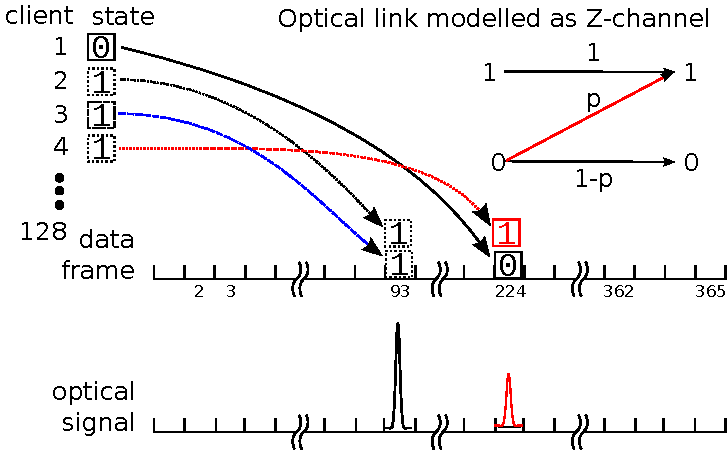
\includegraphics[width=8cm]{graphs/slide4.pdf}
    \\ \huge Colisión $\Rightarrow$ \textcolor{red}{Error}
\end{figure}
\end{frame}
%------------------------------------------------------------
\subsection{Filtro de Bloom}
\frame{\tableofcontents[currentsection,currentsubsection]}

\begin{frame}{CDMA + Filtro de Bloom (K=3)}
\begin{figure}[t]
  \centering
    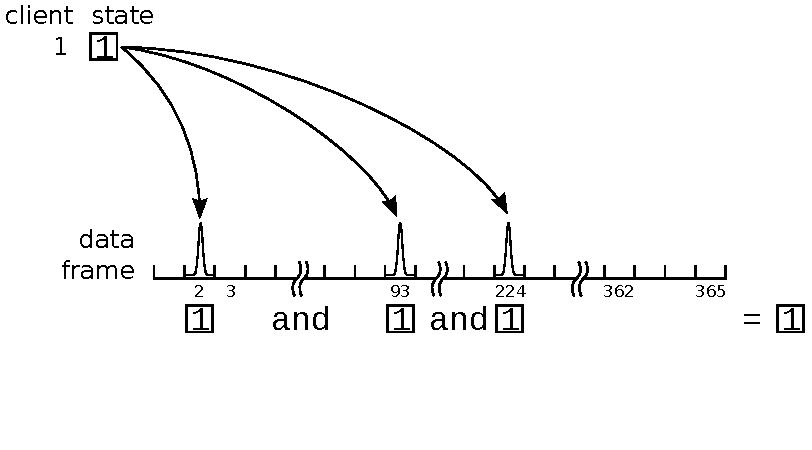
\includegraphics[width=8cm]{graphs/z_bloom1.pdf}
    \\ \huge Inserta el bit '1' en la trama
\end{figure}
\end{frame}
%------------------------------------------------------------
\begin{frame}{CDMA + Bloom filter (K=3)}
\begin{figure}[t]
  \centering
    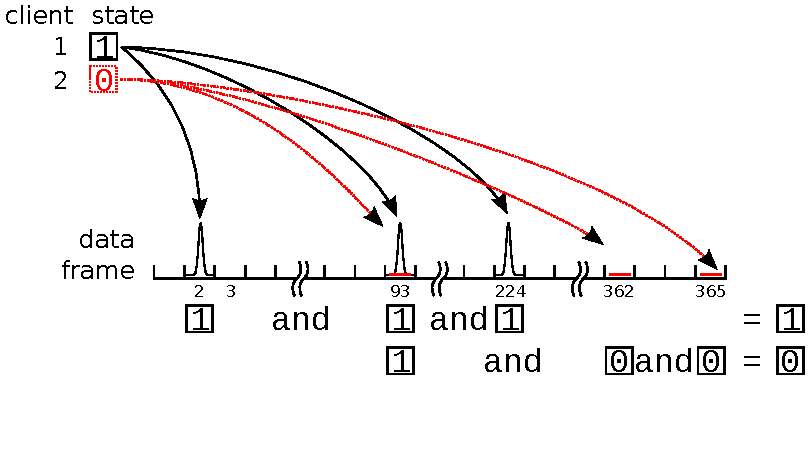
\includegraphics[width=8cm]{graphs/z_bloom2.pdf}
    \\ \huge Inserta el bit '0' en la trama
\end{figure}
\end{frame}
%------------------------------------------------------------
\begin{frame}{CDMA + Bloom filter (K=3)}
\begin{figure}[t]
  \centering
    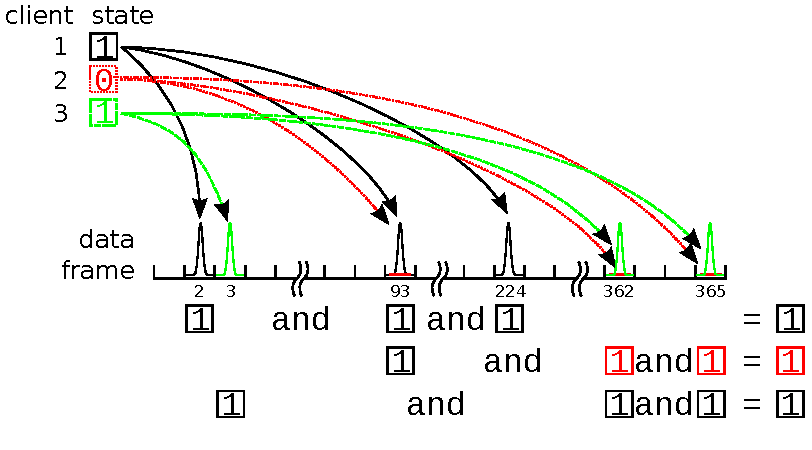
\includegraphics[width=8cm]{graphs/z_bloom3.pdf}
    \\ \huge Inserta el bit '1' en la trama $\Rightarrow$ \textcolor{red}{Error}
\end{figure}
\end{frame}




%------------------------------------------------------------
\subsection{K óptimo}
\frame{\tableofcontents[currentsection,currentsubsection]}

\begin{frame}{K óptimo}



\begin{columns}
  \begin{column}{0.40\textwidth}

  

%\begin{equation}

$\text{BER} \approx \left(1-\left(1-\frac{1}{M}\right)^{N\cdot K\cdot m_1}\right)^K$
%\end{equation}
\vspace{0.5cm}

\begin{itemize}
 \item $M$ es el tamaño de trama.
 \item $N$ es la cantidad de usuarios.
 \item $K$ es el parametró de repetición del filtro de Bloom.
 \item $m_1$ es la cantidad promedio de unos por símbolo.
\end{itemize}

  \end{column}
  \begin{column}{0.60\textwidth}

 

\begin{figure}[!t]
  \centering
    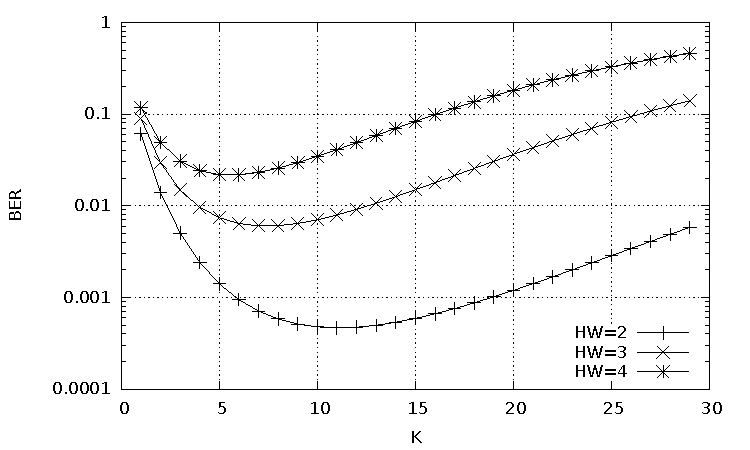
\includegraphics[width=3.5in]{../graphs/calcK}
    
    Estimación del BER en función de $K$ para $M=4096$, $m_{1}$ varía de 2 a 4 y $N=128$.
\end{figure}

  \end{column}
\end{columns}


\end{frame}



%------------------------------------------------------------

\frame{\frametitle{Diagrama esquemático}
\begin{figure}[t]
\centering
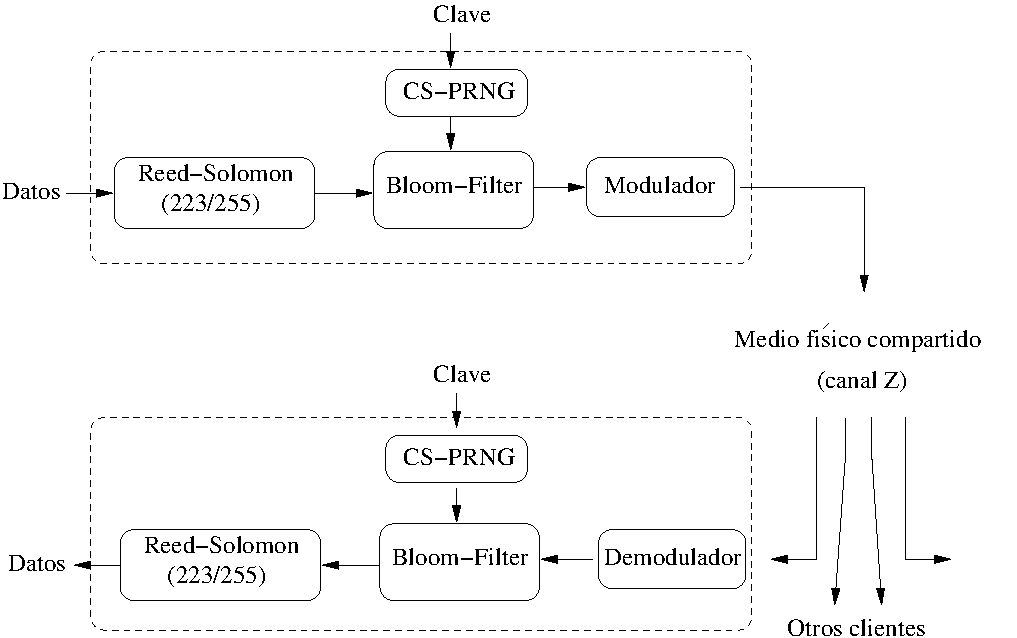
\includegraphics[width=4.5in]{graphs/Soft-stack3}
\label{fig_comstack}
\end{figure}
}

%------------------------------------------------------------

\subsection{Minimización del peso de Hamming}
\frame{\tableofcontents[currentsection,currentsubsection]}

\frame{\frametitle{Minimización del peso de Hamming}
%\framesubtitle{Origen de la técnica}
  \begin{itemize}
  \item Peso de Hamming: cantidad de '1's en un dígito binario.
  \item Ej.: $$HW(00101010) = 3$$
  $$HW(00100000) = 1$$
  \item La minimización del HW es una representación o codificación numérica alternativa. \pause
  \item En un canal Z, los \alert{'1'} producen interferencia, los '0', no. 
  \end{itemize}
}


%------------------------------------------------------------

\frame{\frametitle{Minimización del peso de Hamming}
\framesubtitle{Símbolo de 8-bits, Peso de Hamming=2, expansión a 24 bits}
\begin{center}
\begin{tabular}{c c c}

Dato & Entrada, HW=variable & Expansión HW=2\\
\hline\hline
0 & 00000000 & 00000000000000000\alert{11}\\
1 & 0000000\alert{1} & 0000000000000000\alert{11}0\\
2 & 000000\alert{1}0 & 0000000000000000\alert{1}0\alert{1}\\
3 & 000000\alert{11} & 000000000000000\alert{11}00\\
4 & 00000\alert{1}00 & 000000000000000\alert{1}0\alert{1}0\\
253 & \alert{111111}0\alert{1} & \alert{1}00\alert{1}000000000000000\\
254 & \alert{1111111}0 & \alert{1}0\alert{1}0000000000000000\\
255 & \alert{11111111} & \alert{11}00000000000000000
\end{tabular}
\end{center}

El peso de Hamming fijo previene ataques estadísticos en los datos codificados.

%Example Hamming minimisation table for a 3-bit input symbol with variable hamming weight,
%output is a 5-bit expanded symbol with fixed Hamming weight HW=2
}




%-------------------------------------------------------------
\subsection{Simulaciones}
\frame{\tableofcontents[currentsection,currentsubsection]}

\begin{frame}{Simulaciones: software de prueba}


  \begin{itemize}
  \item Framework de pruebas: Se implementó un módulo independiente por cada etapa.
  \item Utilizado C, C++ y Boost para mejor desempeño.
  \item Incluye un simulador de ruido óptico.
  \item Modulador/demodulador de audio.
  \item Modelo cliente/servidor para simulaciones distribuidas.
  \end{itemize}


\end{frame}

\begin{frame}{Simulación: software de prueba}

  \begin{figure}[t]
    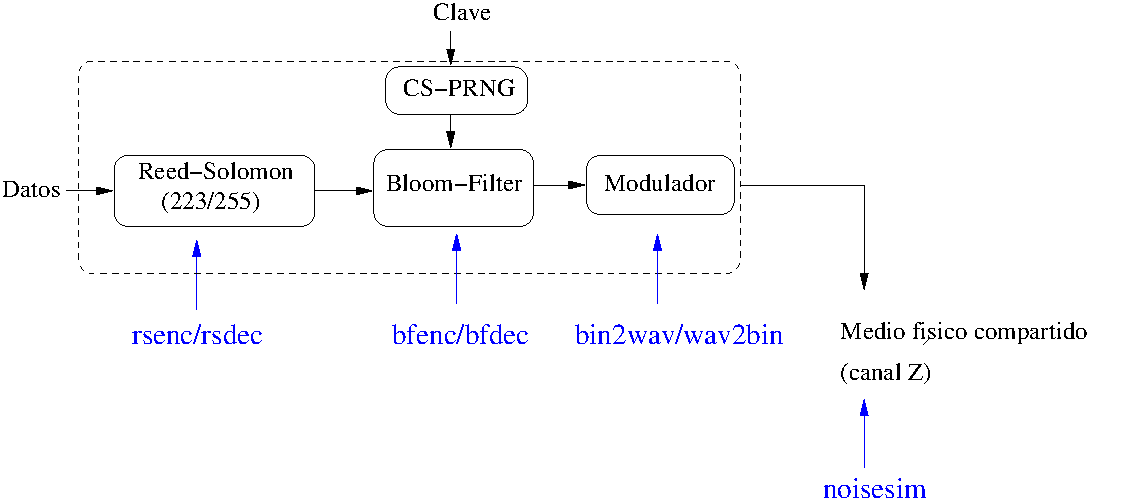
\includegraphics[width=0.90 \textwidth]{../graphs/Soft-stack-sim} 
    
    Correspondencia de etapa con módulos de simulación
\end{figure}


\end{frame}

\begin{frame}[fragile]{Simulación: software de prueba}

Ejemplo de linea de comando para lanzar la simulación:

\small
\begin{verbatim}
 ./rsenc <testfile.in | ./scrambler ${SCRAMBLEBLOCK} >rs.out
 ./bfenc ${CLIENTES} < rs.out | ./noisesim -c ${CLIENTES} -r 16.6 >bfenc.out
 ./bfdec ${CLIENTES} <bfenc.out >bf.out
 ./descramble ${SCRAMBLEBLOCK} <bf.out | ./rsdec >rsdec.out
\end{verbatim}
\normalsize

El BER (\textit{bit error rate}) se calcula con la diferencia entre \textbf{testfile.in} y \textbf{rsdec.out}.
\end{frame}
%-------------------------------------------------------------

\section{Implementación y mediciones}
\subsection{Fibra óptica}
\frame{\tableofcontents[currentsection,currentsubsection]}


\begin{frame}{Implementación sobre red \color{red}óptica}

\begin{columns}
  \begin{column}{0.50\textwidth}

\begin{itemize}
 \item Capaz de operar a 5 Gbps+
 \item Distancias hasta 10 km del nodo central (sin amplificación).
 \item Hasta 128 usuarios simultaneos.
 \item Diseño digital \textit{custom} sobre FPGA.
 \item Utiliza transceptores ópticos SFP+ estandard
 \end{itemize}

  \end{column}
  \begin{column}{0.50\textwidth}

 
\begin{figure}[t]
  \centering
  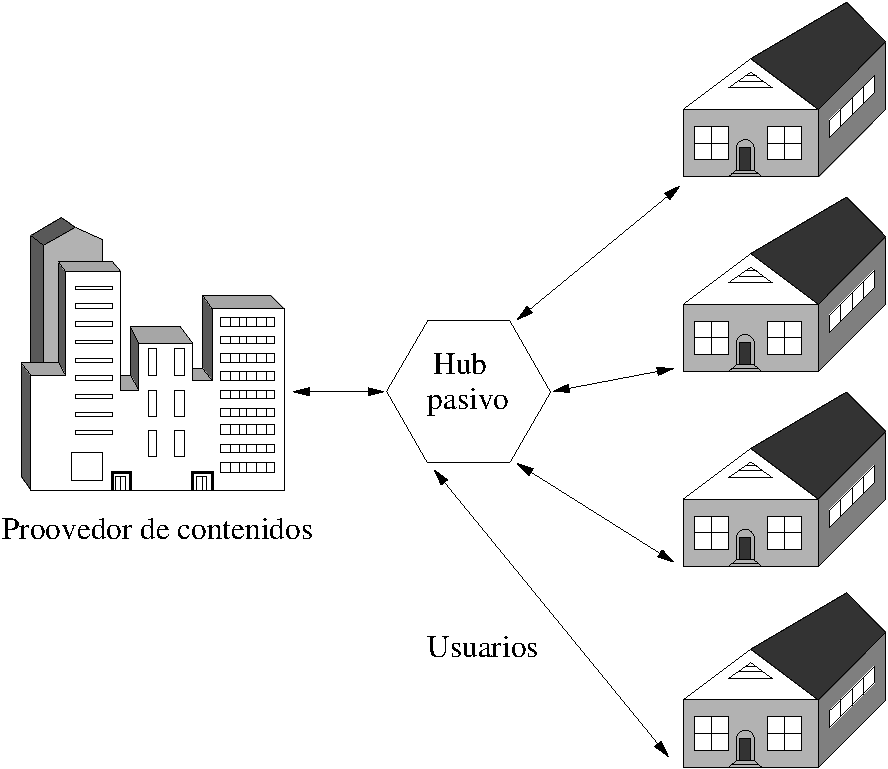
\includegraphics[width=0.85 \textwidth]{../graphs/ftth.pdf} 
\end{figure}

  \end{column}
\end{columns}


\end{frame}

%------------------------------------------------------------

\begin{frame}{Implementación: Fibra óptica}

\begin{figure}[t]
  \centering
      \subfloat[Distribución via acoplador tipo estrella 1]{{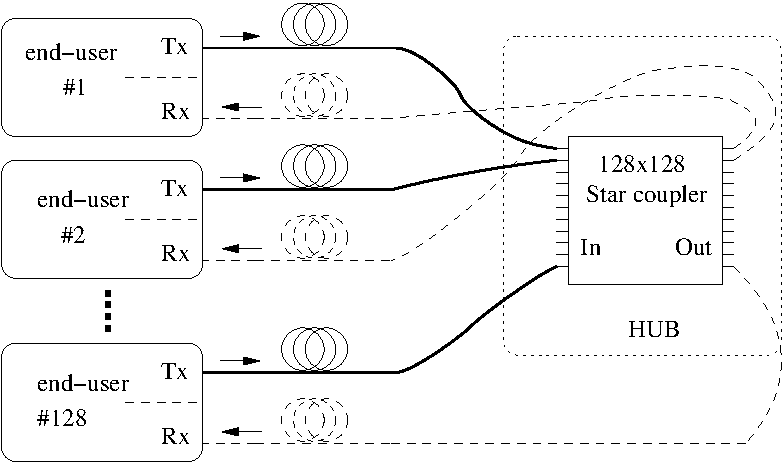
\includegraphics[width=0.4 \textwidth]{graphs/StarCoupler} }}%
    \qquad
    \subfloat[Distribución via EDFA]{{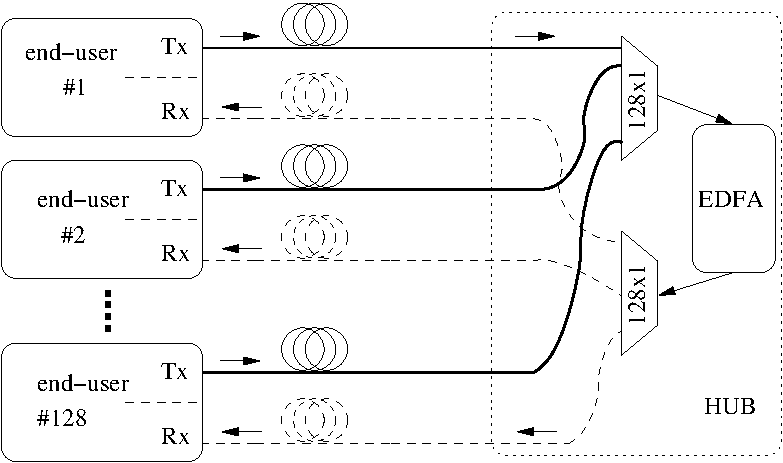
\includegraphics[width=0.4 \textwidth]{graphs/EDFA} }}%
    
    Diseño de red propuesto para la capa óptica
    \label{arch:fig1}
\end{figure}

\end{frame}

%-------------------------------------------------------------
\begin{frame}{Implementación: Fibra óptica, Resultados (Simulaciones)}

\begin{figure}[!t]
  \centering
    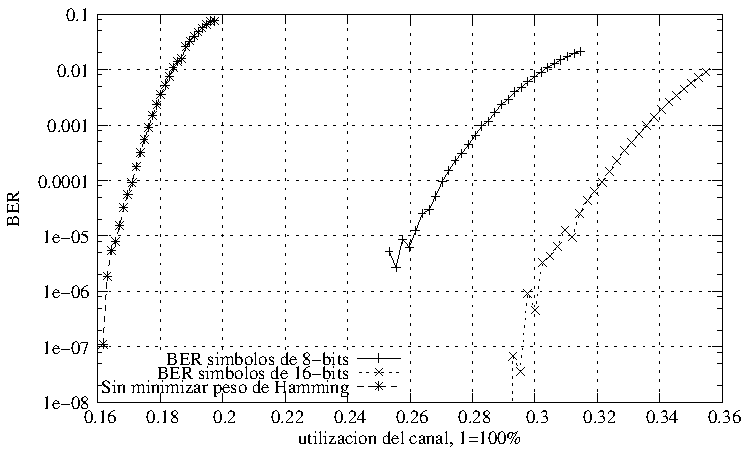
\includegraphics[width=4in]{../graphs/BERvsChannelES2}
    
    Desempeño del sistema con respecto a la expansión de símbolo. Simulación numérica de un enlace de 10 Gbps con 128 clientes, M=4096 y K=9.
    \label{BERvsExpansion}
\end{figure}

\end{frame}

%-------------------------------------------------------------
\begin{frame}{Implementación: Fibra Óptica}

\framesubtitle{Placas de desarrollo Xilinx ML507}
  \centering
  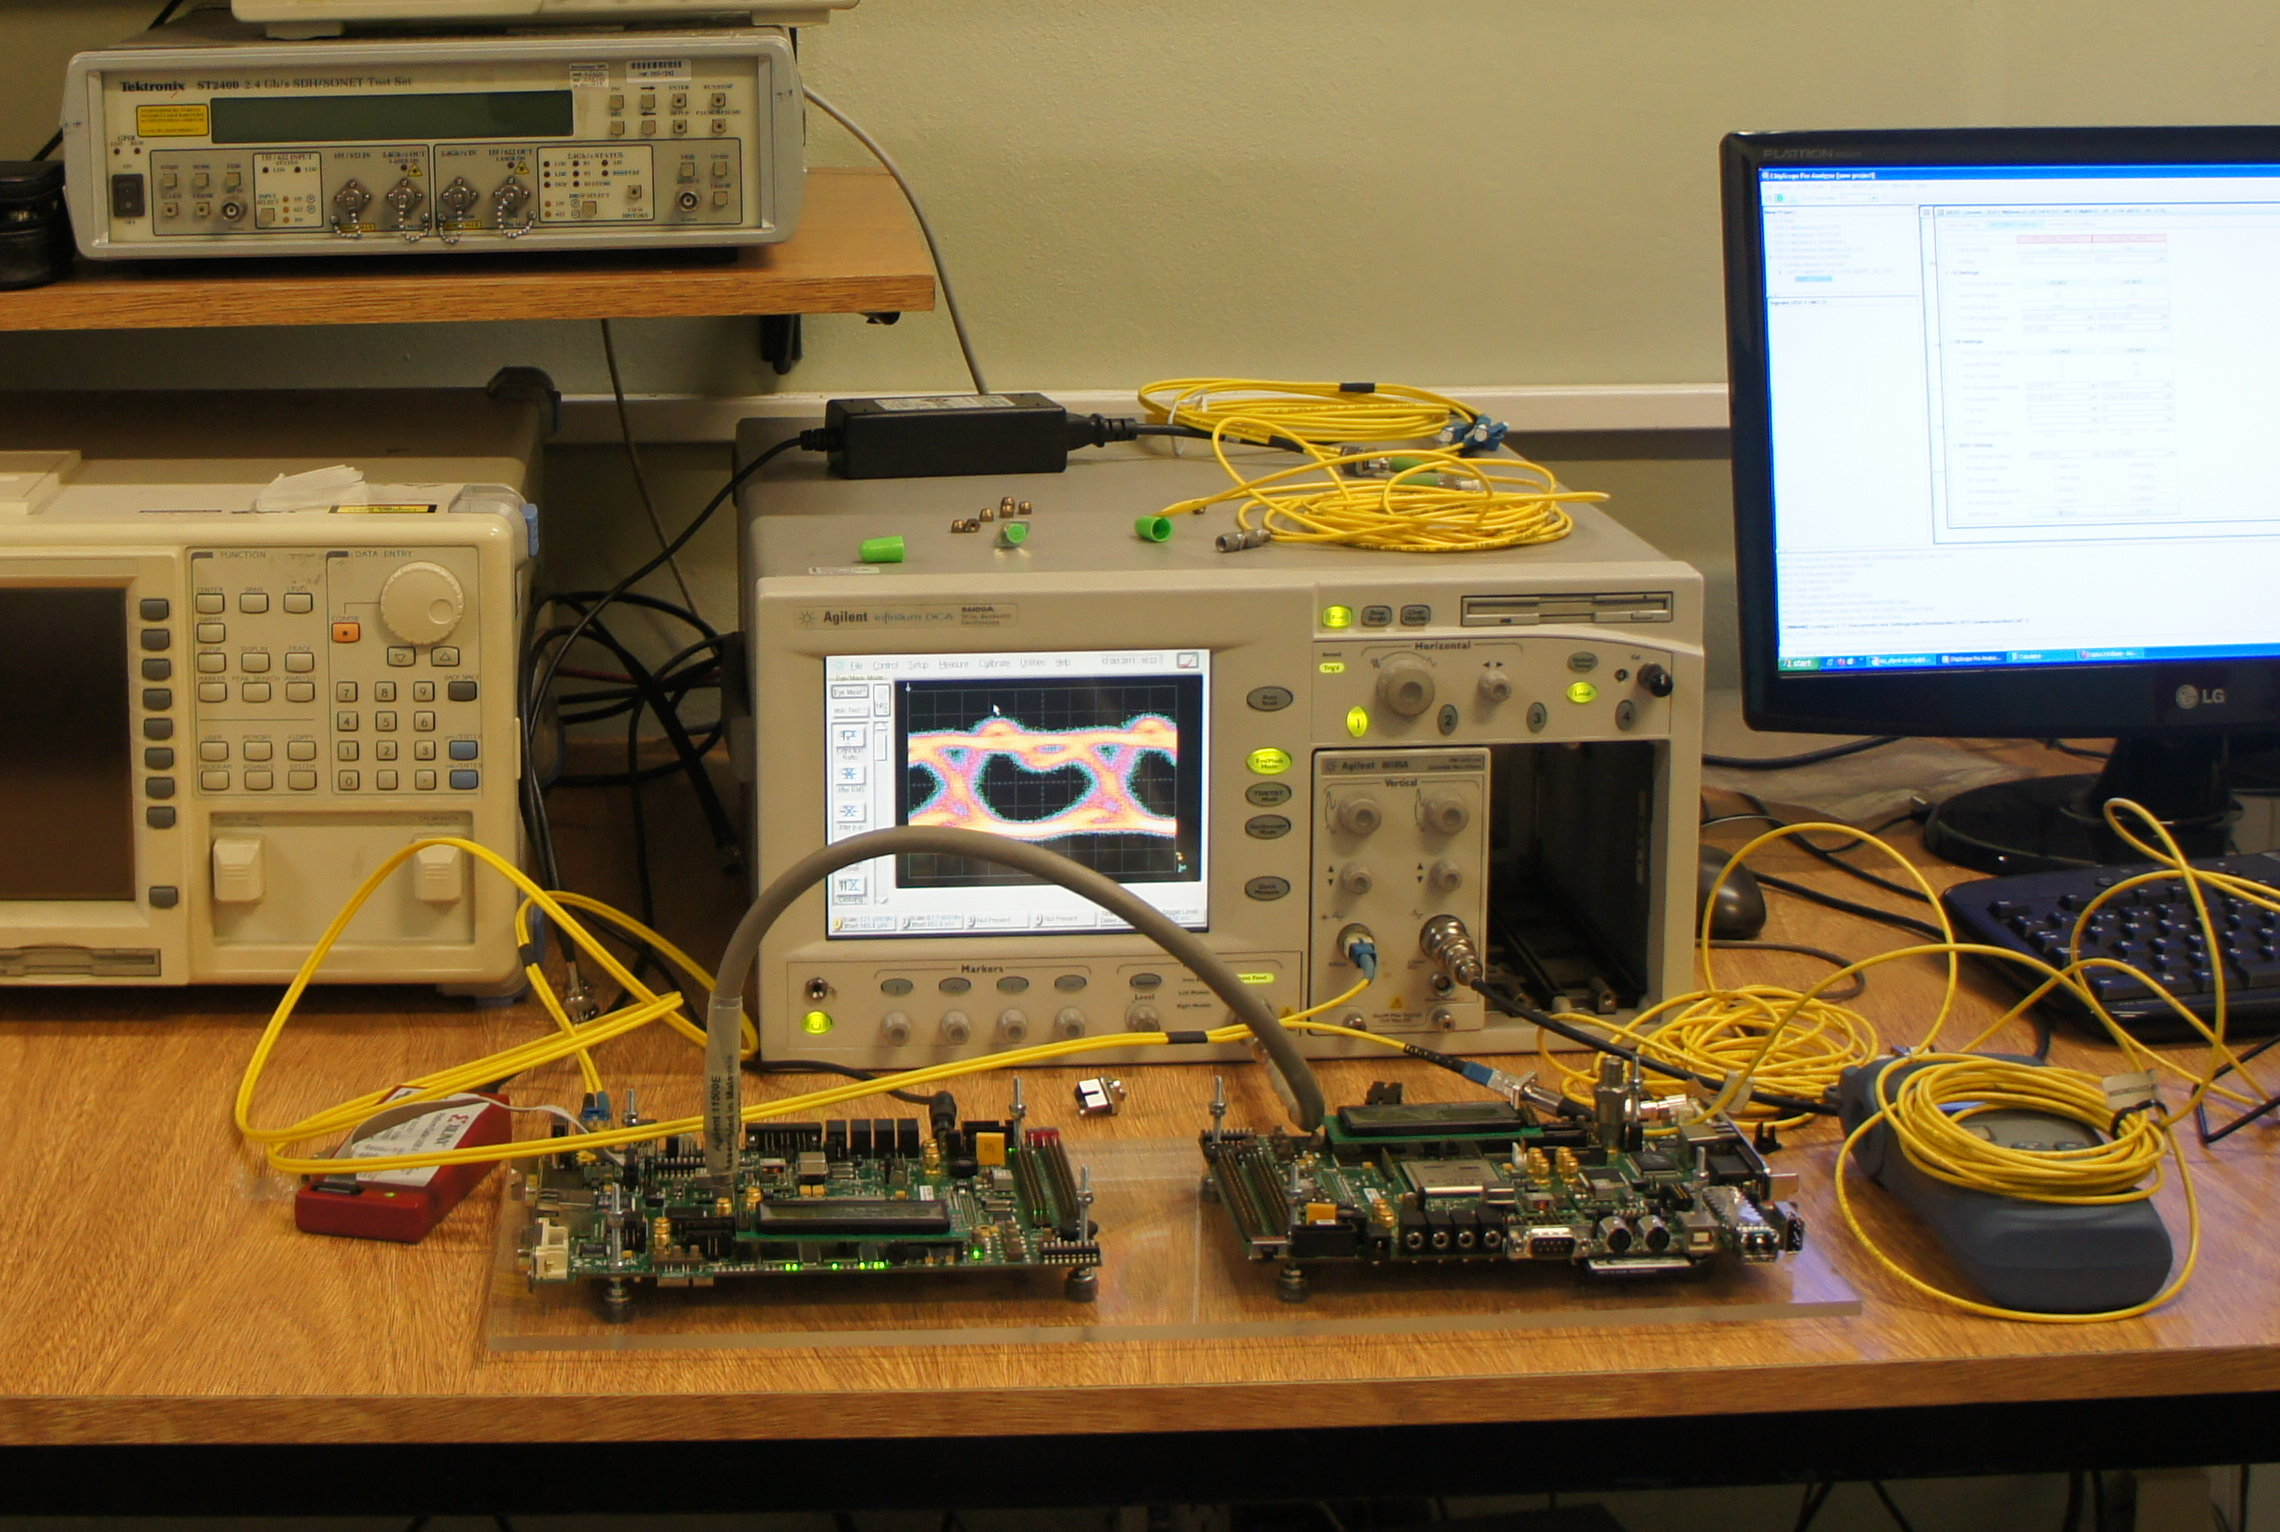
\includegraphics[width=0.7\textwidth]{graphs/fpga.jpg} 

\end{frame}



%-------------------------------------------------------------
\begin{frame}{Implementación: Fibra óptica, FPGA}


\begin{columns}
  \begin{column}{0.35\textwidth}

   
\begin{itemize}
 \item CPU Microblaze (Debugging), 75 Mhz, sin DRAM
 \item Coprocesador, 100 Mhz
 \item Utilización (\textit{Slices}): 9446 de 11200, \alert{84\%}
 \item Tiempo de sintetizado: aprox. 40 minutos (Core i7 2da generación)
 
 \end{itemize}

  \end{column}
  \begin{column}{0.65\textwidth}

  \begin{figure}[t]
  \centering
    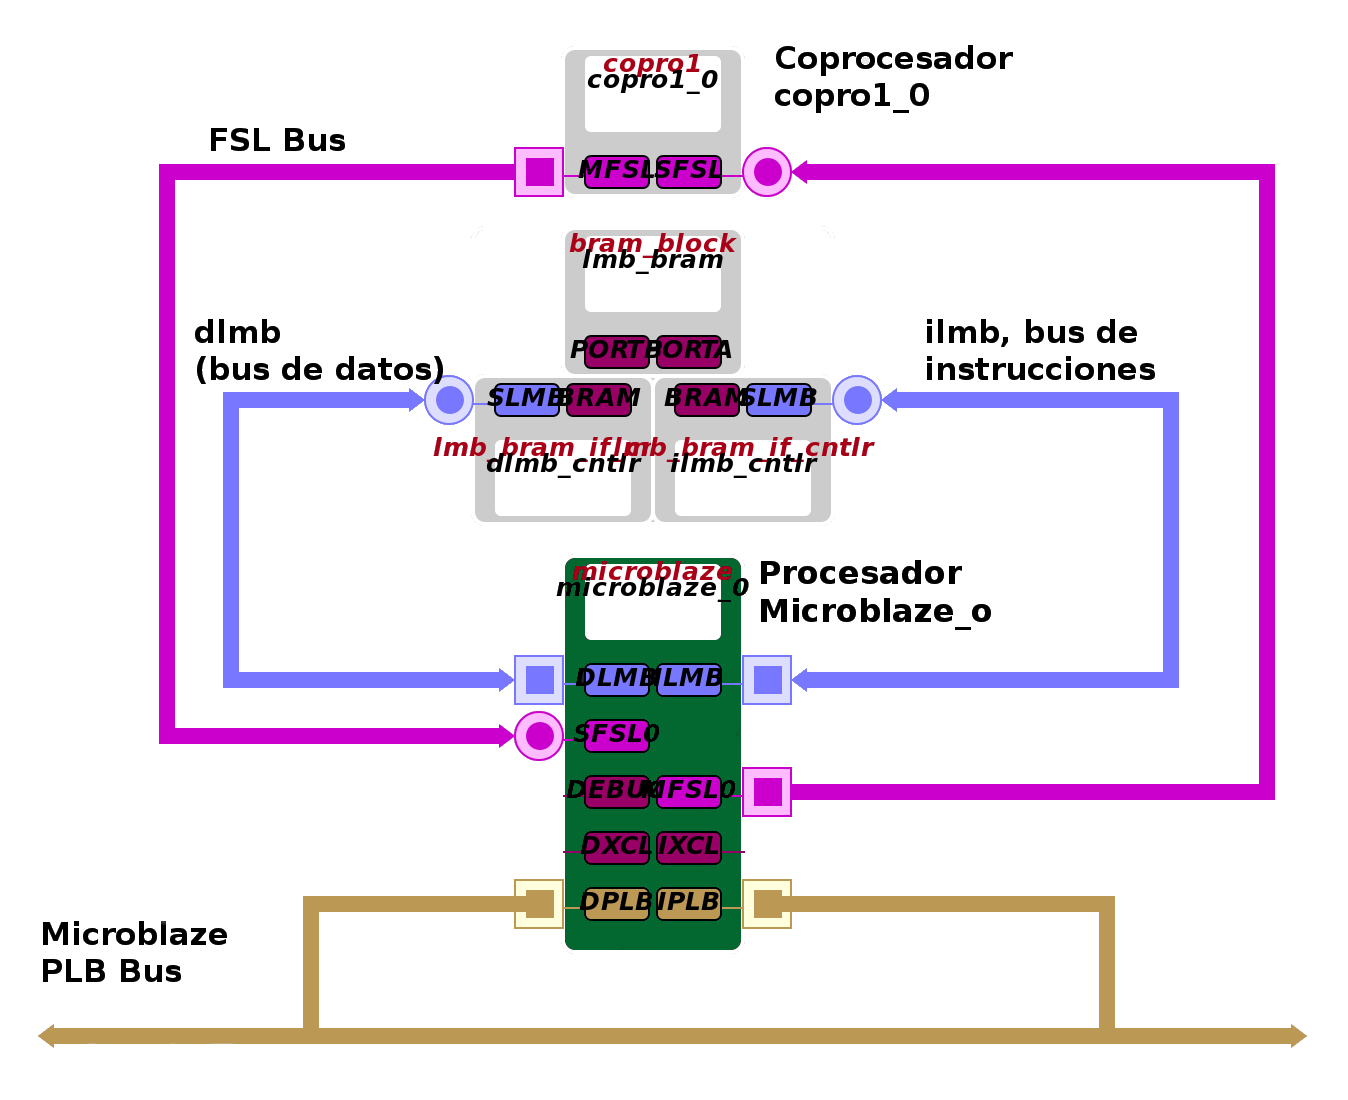
\includegraphics[width=3.5in]{../graphs/diagramaXilinx.png}
\label{fig:fpgahard}
\end{figure}

  \end{column}
\end{columns}



\end{frame}


%-------------------------------------------------------------
\begin{frame}{Implementación: Fibra óptica, FPGA}

 \begin{figure}[t]
  \centering
    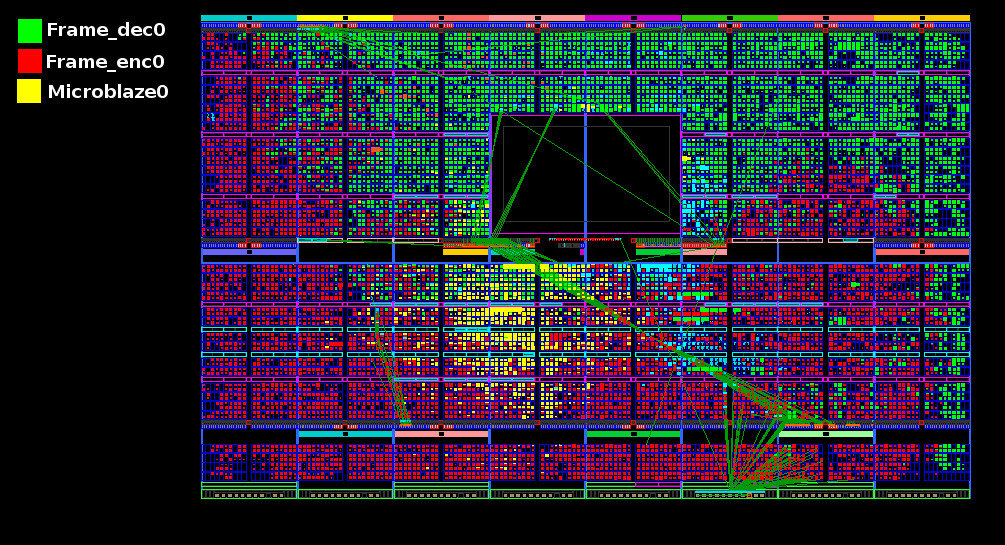
\includegraphics[width=5.5in]{graphs/fpgamap.jpg}
\label{fig:fpgahard}
\end{figure}


\end{frame}



%-------------------------------------------------------------
\begin{frame}{Implementación: Efectos de señal desbalanceada}


\begin{figure}[!t]
   \centering
   \subfloat[Señal con 256 bits en uno por trama (8B/10B), 400 ps por bit]{{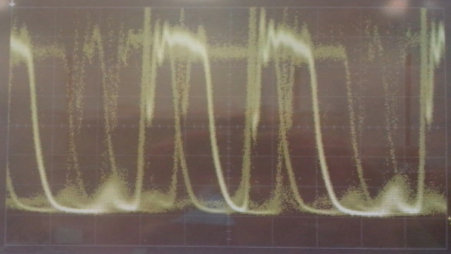
\includegraphics[width=0.45 \textwidth]{../graphs/expansion1.jpg} }}%
   \qquad
   \subfloat[Señal con 48 bits en uno por trama, 1100 ps por bit]{{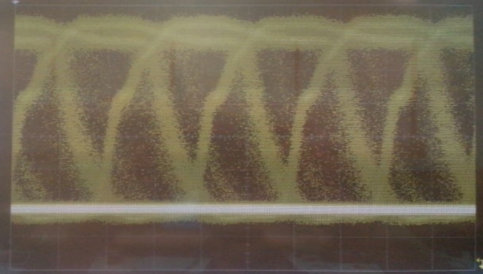
\includegraphics[width=0.45 \textwidth]{../graphs/expansion2.jpg} }}%
   \qquad
   
  \vspace{0.2cm}
  Señal de potencia óptica de un Láser SPF+ de 1330 nm, tasa nominal es de 2.5 Gbps.
  \label{fig:ImgExpansion}
\end{figure}
\end{frame}

%-------------------------------------------------------------
\begin{frame}{Mediciones ópticas}


\begin{columns}
  \begin{column}{0.40\textwidth}

\begin{itemize}
\item Atenuador fijo en 10.85 DB
\item Velocidad de enlace: 2.5 gbps
\item SFP de link: sumitomo-electric-scp681 (S-16.1DDM)
\item SFP de ruido: sumitomo-electric-scp681 (L-16.1)
 \end{itemize}

  \end{column}
  \begin{column}{0.70\textwidth}

\begin{figure}[!t]
   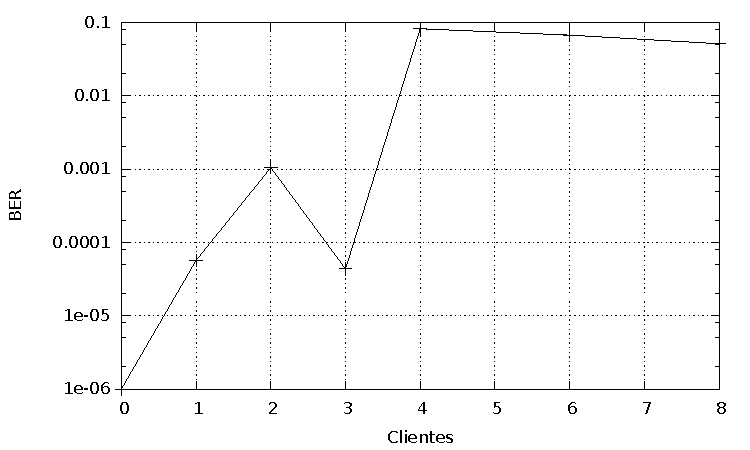
\includegraphics[width=0.90 \textwidth]{graphs/medicion-optica-ber-sumitomo}
   \qquad
   
  \vspace{0.2cm}
  BER antes de corrección de errores
\end{figure}

  \end{column}
\end{columns}



\end{frame}

%------------------------------------------------------------
\subsection{Medio acústico}
\frame{\tableofcontents[currentsection,currentsubsection]}


\begin{frame}{Implementación sobre red \color{red}acústica}

\begin{columns}
  \begin{column}{0.50\textwidth}

\begin{itemize}
 \item Modem: 1 Khz de ancho de banda, 1 Kbps, portadora a 12 Khz y 16 Khz (inaudible).
 \item Distancias hasta 2 m del nodo central.
 \item Máximo de 8 usuarios.
 \item Implementación puramente en software.
 \item Utiliza hardware existente en celulares y notebooks (micrófonos y parlantes).
 \end{itemize}

  \end{column}
  \begin{column}{0.50\textwidth}

 
\begin{figure}[t]
  \centering
  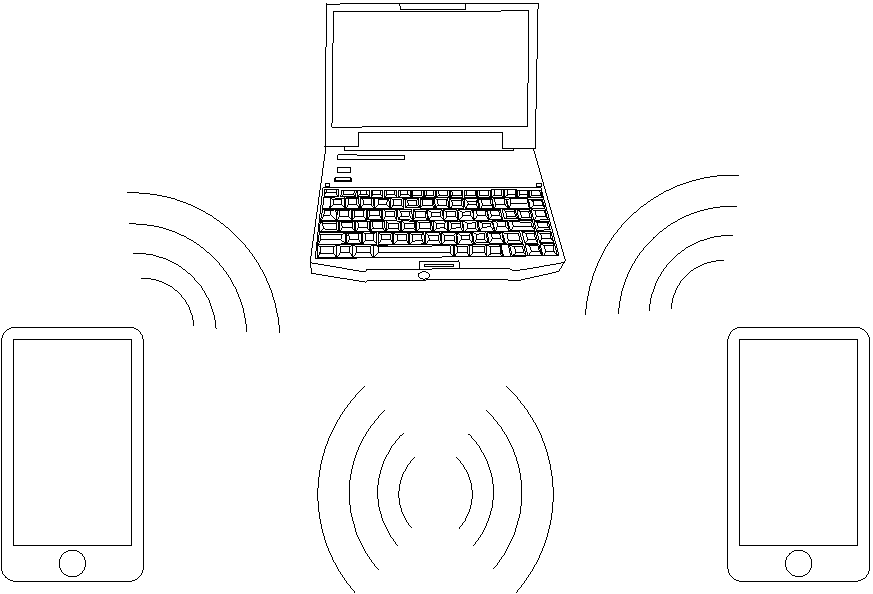
\includegraphics[width=0.85 \textwidth]{../graphs/compucelus.pdf}
\end{figure}

  \end{column}
\end{columns}

\end{frame}



%------------------------------------------------------------
\begin{frame}{Medio acústico: modulación}

\begin{columns}
  \begin{column}{0.40\textwidth}

  \begin{figure}[t]
  \centering
    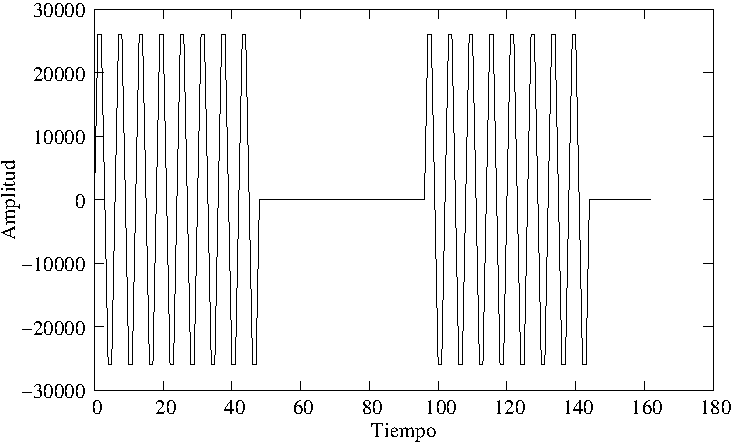
\includegraphics[width=5cm]{graphs/modulated.pdf}
    
    Modulación OOK.
    \label{arch:sync}
\end{figure}

  \end{column}
  \begin{column}{0.50\textwidth}
\begin{figure}[th]
  \begin{center}
    \vspace{0.7cm}
    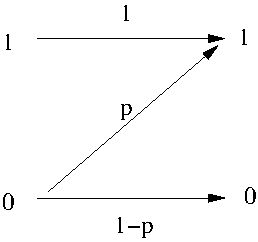
\includegraphics[width=3cm]{../graphs/zchannel}
    
    Diagrama de probabilidad: canal Z.
  \end{center}
  \label{fig:Gal}
\end{figure}

  \end{column}
\end{columns}
\vspace{0.2cm}

\begin{itemize}
 \item Interferencia de OOK se aproxima a la de un canal Z.
 \item Baja densidad espectral (0.2 bits/s/Hz)
\end{itemize}

\end{frame}
%------------------------------------------------------------

\begin{frame}{Medio acústico: sincronización}

\begin{figure}[t]
  \centering  
    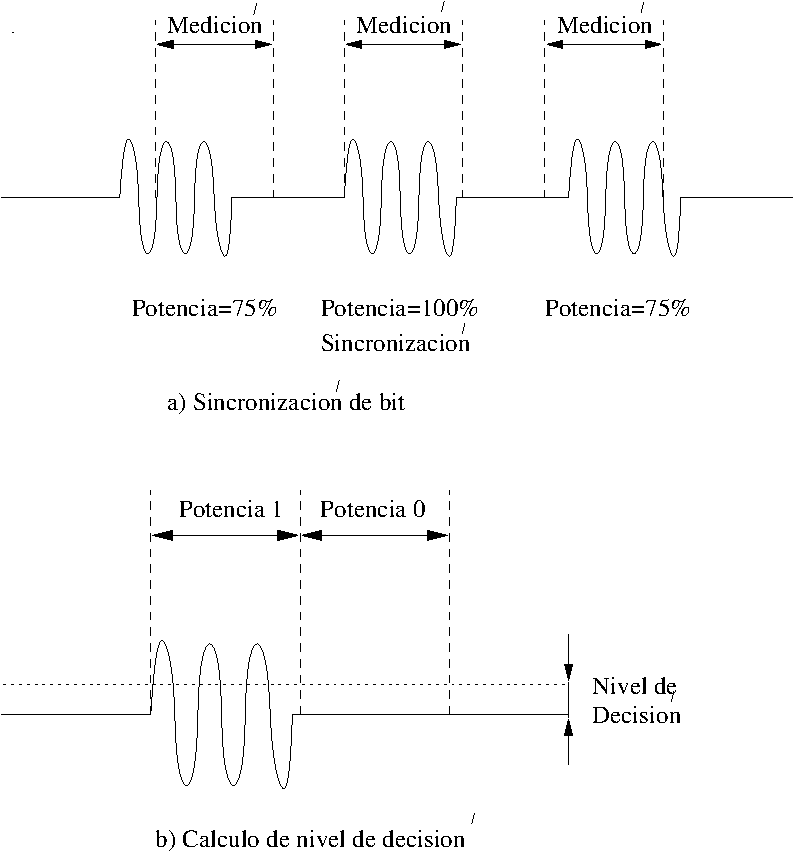
\includegraphics[width=6cm]{graphs/acusync}
    \\ Sincronización de bit/nivel de decisión
    \label{ios_process_mem}
\end{figure}

\end{frame}
%------------------------------------------------------------

\begin{frame}{Medio acústico: características y espectro}

\begin{figure}[t]
  \centering  
    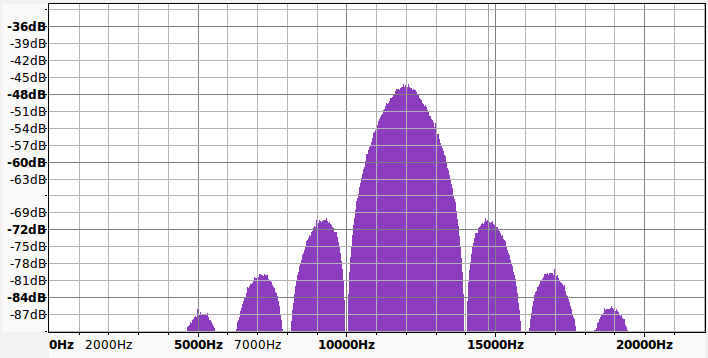
\includegraphics[width=10cm]{graphs/spectrum.png}
    \\ Espectro de señal modulada, salida directa del modem.
    \label{ios_process_mem}
\end{figure}

\begin{itemize}
 \item Portadora a 12 Khz, modem funcionando a 1 Kbps en total
 \item Velocidades de 350 bps (2 usuarios) a 70 bps (10 usuarios)
 \item Dispositivos móviles: buen desempeño parlante/micrófono de 100 a 15 Khz
\end{itemize}

\end{frame}

%------------------------------------------------------------
\begin{frame}{Medio acústico: resultados (simulaciones y mediciones)}
  
  \begin{figure}[t]
  \centering  
    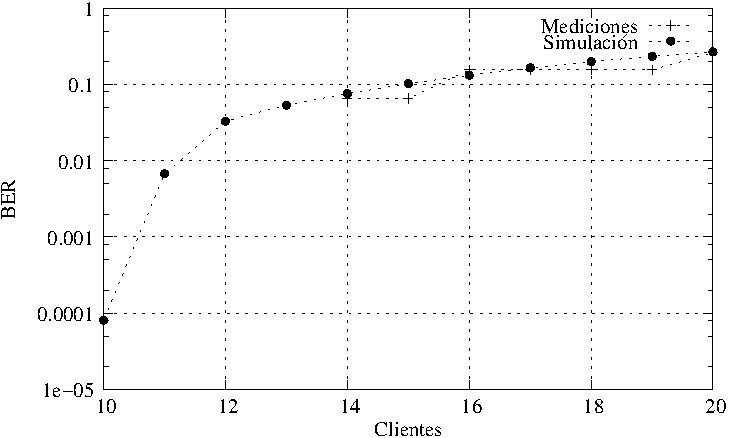
\includegraphics[width=8cm]{graphs/medidas_clientes_JIS-fig6}
    \\ BER $vs.$ número de clientes
    \label{ios_process_mem}
\end{figure}

\end{frame}

%------------------------------------------------------------
\begin{frame}{Medio acústico: resultados (mediciones)}
  
\begin{figure}[t]
  \centering  
    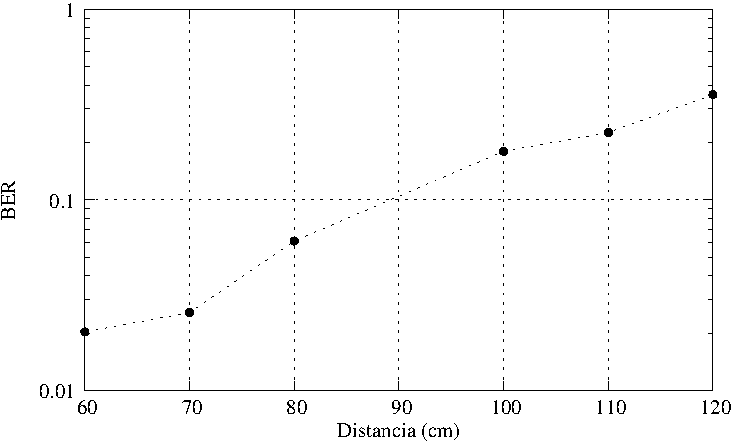
\includegraphics[width=8cm]{graphs/mediciones-distancia-fig7}
    \\ BER $vs.$ distancia
    \label{ios_process_mem}
\end{figure}

\end{frame}


%-------------------------------------------------------------

\section{Conclusiones}
\frame{\tableofcontents[currentsection]}

\frame{\frametitle{Conclusiones:}
\begin{itemize}
\item Se propuso una arquitectura de red privada tipo \alert{time-hopping CDMA}:\pause\vfill
  \begin{itemize}
  \item Para redes de difusión del tipo \alert{canal z}.\pause\vfill
  \item Utilizando \alert{filtros de Bloom} y minimización de peso de \alert{Hamming}.\pause\vfill
  \item Punto-a-Punto, y Punto-a-\alert{Multipunto}.\pause\vfill
  \item {\bf 29\% de utilización del canal.} \vfill
  \end{itemize}
\end{itemize}
}

%-------------------------------------------------------------
\frame{\frametitle{Trabajos futuros:}
  \begin{itemize}
  \item Sincronización segura.
  \item Encriptación autenticada.
  \item Autenticación de nodos y distribución de claves (\textit{Forward Secrecy}).
  \item Implementación en otros medios. Ej. Radio.
  \end{itemize}
  
}


%-------------------------------------------------------------
\begin{frame}{Contribuciones:}
%\small
\textbf{Altas velocidades de transferencia en fibra óptica utilizando FPGAs de bajo costo. } \textit{A. A. Ortega, V. A. Bettachini, D.F. Grosz, J. I. Alvarez-Hamelin - Congreso de Microelectrónica Aplicada 2010 BsAs}

\

\textbf{ Point-to-point and Point-to-multipoint CDMA Access Network with Enhanced Security} \textit{ A. A. Ortega, V. A. Bettachini, J. I. Alvarez-Hamelin,  D.F. Grosz, Advanced Photonics 2011 Congress - Access Networks and In-house CommunicationsAccess Networks and In-house Communications, OSA Technical Digest, Optical Society of America}

\

\textbf{Hamming-weight minimisation coding for CDMA optical access networks with enhanced security} \textit{ A. A. Ortega, V. A. Bettachini, J. I. Alvarez-Hamelin, D.F. Grosz, Future Generation Communication Technology (FGCT), 2012}


\end{frame}


\begin{frame}{Contribuciones:}
%\small
\textbf{Encrypted CDMA Audio Network.} \textit{ A. A. Ortega, V. A. Bettachini, P. I. Fierens, y J. I. Alvarez-Hamelin -  Journal of Information Security - 2014}

\

\textbf{Patente: DISPOSITIVO Y MÉTODO PARA TRANSMISIÓN SEGURA DE DATOS SOBRE CANALES Z MEDIANTE CDMA (AR084155B1)}\textit{José Ignacio ALVAREZ HAMELIN, Victor Alexis BETTACHINI, and Alfredo ORTEGA. PCT, 12 2012. (Asignada)}

\

\textbf{Patente: Device and Method for the Secure Transmission of Data over Z-Channels Using CDMA (P11104EPPC)}\textit{José Ignacio ALVAREZ HAMELIN, Victor Alexis BETTACHINI, and Alfredo ORTEGA. EPO, Julio 2014. (En trámite)}

\
\end{frame}

\frame{\frametitle{Fin de la presentación}

Muchas gracias por su asistencia.

}

%-------------------------------------------------------------

\footnotesize

\begin{thebibliography}{7}


\providecommand{\natexlab}[1]{#1}
\providecommand{\url}[1]{\texttt{#1}}
\expandafter\ifx\csname urlstyle\endcsname\relax
  \providecommand{\doi}[1]{doi: #1}\else
  \providecommand{\doi}{doi: \begingroup \urlstyle{rm}\Url}\fi


\bibitem[Mosso et~al.(2011)]{mosso2011all}
F.~Mosso, J.~Barrera, M.~Tebaldi, N.~Bolognini, and R.~Torroba.
\newblock All-optical encrypted movie.
\newblock \emph{Opt. Express}, 19\penalty0 (6):\penalty0 5706--5712, 2011.

\bibitem[Nadarajah et~al.(2006)]{Nadarajah2006}
N.~Nadarajah, E.~Wong, and a.~Nirmalathas.
\newblock {Implementation of multiple secure virtual private networks over
  passive optical networks using electronic CDMA}.
\newblock \emph{IEEE Photonics Technology Letters}, 18\penalty0 (3):\penalty0
  484--486, Feb. 2006.
\newblock ISSN 1041-1135.
\newblock \doi{10.1109/LPT.2005.863637}.
\newblock URL
  \url{http://ieeexplore.ieee.org/lpdocs/epic03/wrapper.htm?arnumber=1576846}.


\bibitem[Shake(2005)]{Shake:05}
T.~Shake.
\newblock Security performance of optical cdma against eavesdropping.
\newblock \emph{IEEE Journal of Lightwave Technology}, 23:\penalty0 655--670,
  Feb. 2005.

\bibitem[Torres et~al.(2002)]{torres2002}
P.~Torres, L.~Valente, and M.~Carvalho.
\newblock Security system for optical communication signals with fiber bragg
  gratings.
\newblock 50:\penalty0 13--16, Jan. 2002.

\bibitem[Jay, John A]{jay2010}
Jay, John A., An overview of macrobending and microbending of optical fibers.
\newblock \emph{White Paper WP1212, Corning}, 2010.



\end{thebibliography}


\end{document}


